\section{Ingestion module for the REP\_SUP file}
This section describes the ingestion module of the REP\_\acrshort{sup} reports, which are generated by \acrshort{fos} and contain information about the satellite unavailabilities.

The associated ingestion processors are:

\begin{itemize}

\item \textbf{s2boa.ingestions.ingestion\_sup.ingestion\_sup} 

\end{itemize}

This module use the following \acrshort{dim} signatures:

\begin{itemize}

\item \textbf{SATELLITE\_UNAVAILABILITY}: information about the satellite's subsystems unavailabilities. 
    
\end{itemize}

The table \ref{tb:description_events_ingestion_sup} shows the description of the events inserted by the ingestion.

\begin{landscape}
\begin{longtable}{|M{0.09\linewidth}|M{0.05\linewidth}|M{0.10\linewidth}|M{0.12\linewidth}|M{0.09\linewidth}|M{0.09\linewidth}|M{0.09\linewidth}|}
\hline \textbf{Gauge name} & \textbf{Gauge system} & \textbf{DIM signature} & \textbf{Insertion mode} & \textbf{Description} & \textbf{Start} & \textbf{Stop} \\ \hline
\textbf{SATELLITE\_UNAVAILABILITY} & XXX & SATELLITE\_UNAVAILABILITY & EVENT\_KEYS (insert) [KEY: XXX-SUBSYSTEM-REFERENCE] & Event for representing the \textbf{unavailability impact.} & UTC start time value inside the subsystem node & UTC end time value inside the subsystem node  \\ \hline
\caption{Table describing the events associated to the ingestion}
\label{tb:description_events_ingestion_sup}
\end{longtable}
\end{landscape}

Where XXX is the corresponding satellite id, SUBSYSTEM is the name of the impacted satellite subsystem and REFERENCE is the unavailability reference for the impact on the given subsystem.

The figure \ref{fg:structure_ingestion_sup_events} shows a simplified diagram of the structure of events inserted (associated structure of values not included for simplicity).

\begin{figure}[H]
  \begin{center}
	\centering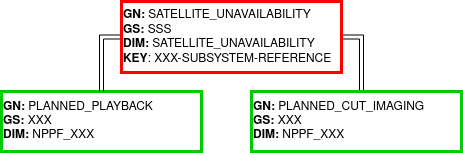
\includegraphics[scale=0.7]{../fig/structure_ingestion_sup.png}
	\caption{Structure of events inserted by the ingestion module for the REP\_\acrshort{sup} file}
	\label{fg:structure_ingestion_sup_events}
  \end{center}
\end{figure}

Where the inserted event will be only linked to one of the two included events (PLANNED\_PLAYBACK or PLANNED\_CUT\_IMAGING) depending on the impacted subsystem:

\begin{itemize}

\item If the satellite unavailability impacts the MSI or the MMFU subsystems (imaging), then the inserted event will be linked to the PLANNED\_CUT\_IMAGING events.

\item If the satellite unavailability impacts the XBAND or OCP subystems (downlink), then the inserted event will be linked to the PLANNED\_PLAYBACK events.

\end{itemize} 

